\chapter{Data acquisition}

The data used in the paper has been gathered over the course of three months, starting in early March and ending in late May. The data has been obtained with the help of three student volunteers. Each volunteer carried a phone, provided by the SensibleDTU project, the same project this thesis is a part of \cite{sensibledtu, Stopczynski}. The phones are Samsung Galaxy Nexus \cite{nexus} and are running the Android operating system \cite{android}. 

Each phone came with two apps. The first recorded regularly a multitude of information, such as bluetooth RSSI, GPS traces, battery usage and cell tower information, and is a part of the SensibleDTU project \cite{Stopczynski}, while the second allowed the volunteers to manually name the person they are in physical proximity with, and was developed during this thesis. The second app provided the ground-truth information.

This gave rise to two types of data. First, a continuous stream of regular measurements from the first app, and punctual messages from the second app. Below we will go into more detail about how exactly the two types of data look, how are they gathered and finally, how the two are combined to create a unitary set which serves as a basis for the machine learning algorithms.

\section{FriendFinder app}

\subsection{App overview and implementation}

As the app, FriendFinder, is made for the Android operating system, it is implemented using Java for Android \cite{jandroid}. It has a Google App Engine backend \cite{googleapp}. Fig \ref{pic:ff_prtscr} shows the main screen of the app. 

\begin{figure}[h]
	\begin{center}
		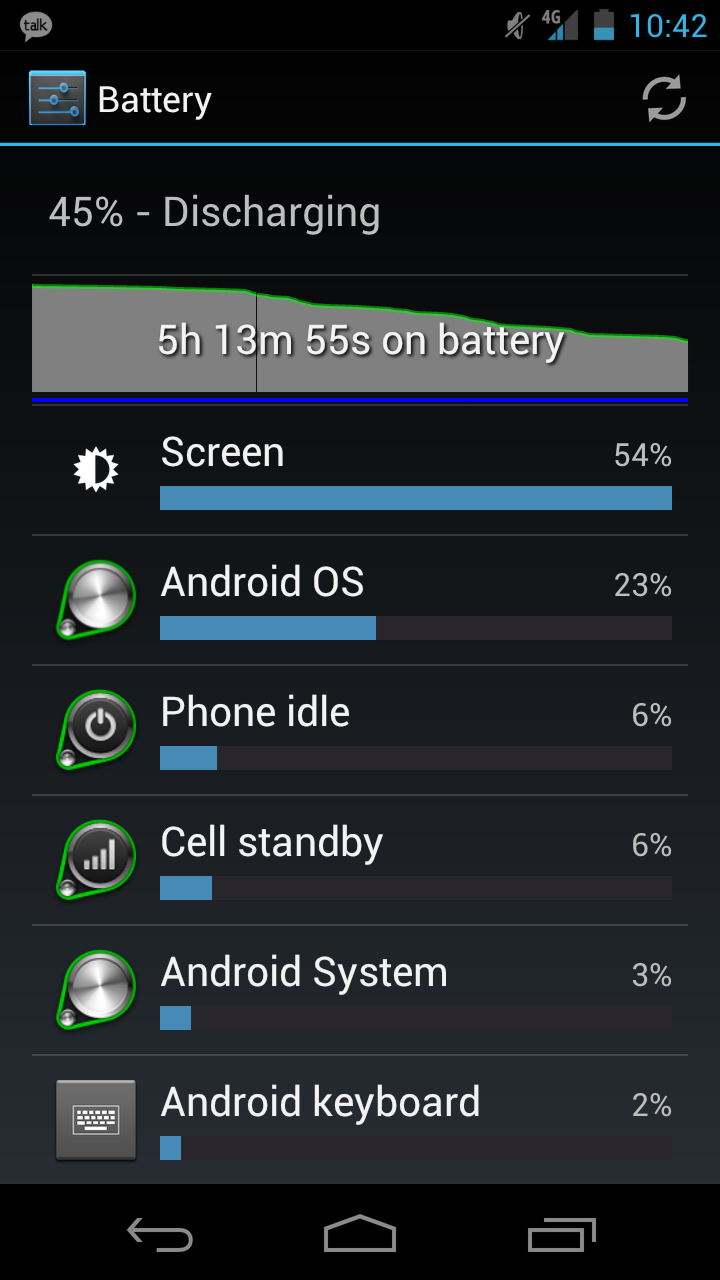
\includegraphics[scale=0.2]{figures/galaxy-nexus-battery.png}
	\end{center}
	
	\caption{FriendFinder app}.
	\label{pic:ff_prtscr}

\end{figure} 

FriendFinder is implemented using a client server architecture, where the clients are the apps installed on the phone, and the server is the Google App Engine. Fig \ref{pic:clientserver} shows an overview of this particular architecture. In this case, the FriendFinder app (in the role of the client) makes a \textit{save data} request to the Google App Engine (the server). The server in turn responds with the result of the operation, either a \textit{succes} or \textit{failure} message.  

\begin{figure}[h]
	\begin{center}
		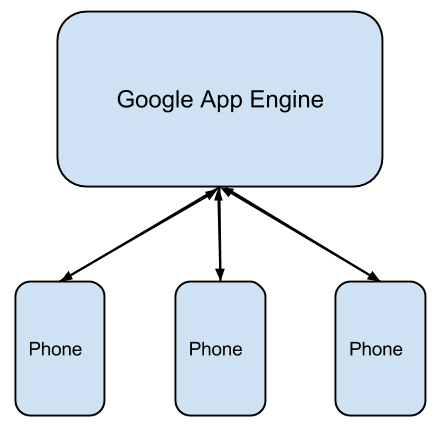
\includegraphics[scale=0.5]{figures/SC_Arch.png}
	\end{center}
	
	\caption{Client Server Architecture used by the FriendFinder app}.
	\label{pic:clientserver}

\end{figure} 

The app contains a single screen (the one showed in Fig \ref{pic:ff_prtscr}), which corresponds to the main activity. Activities are the main building blocks of an Android app, and they are used both to interact with the user, as well as provide additional functionalities \cite{activity}. On the main screen there are buttons for each volunteer. Once one of the volunteers is in physical proximity with another volunteer (as perceived by either one), they both press the button corresponding to each other. A confirmation message is displayed, as can be seen in Fig. \ref{pic:ff_conf}.

\begin{figure}[h]
	\begin{center}
		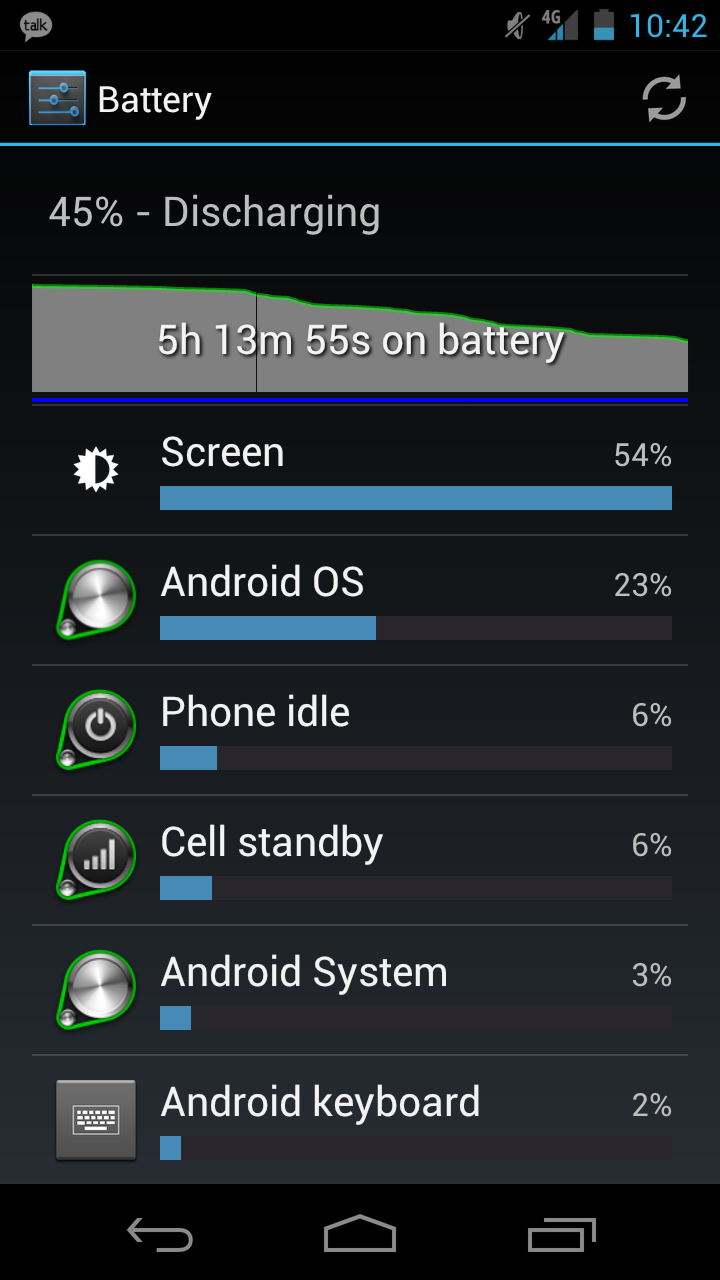
\includegraphics[scale=0.2]{figures/galaxy-nexus-battery.png}
	\end{center}
	
	\caption{Confirmation message on the FriendFinder app}.
	\label{pic:ff_conf}

\end{figure}

For the data to reach the database on the Google App Engine, an internet connection is required. However, the app can also function off-line, by saving all the data locally, and sending it to the on-line database as soon as an internet connection is established. It does this by using an IntentService \cite{intentservice}, which has two main functions:

\begin{itemize}
  \item A first function is to store the data locally, until an internet connection is established.
  \item the second, and most important, is to check periodically for an internet connections. Once an internet connection has been established, all the data is sent to the Google App Engine. The app checks every one minute for internet access. This allows for a relatively fast updating of the database, while at the same time keeping the resource use at a level that does not impede the normal functioning of the phone.
\end{itemize}

The data is stored locally in RAM of the phone (the volatile memory). This is made possible by the relatively small size of the data being saved ( the names of the two people involved, and an ID object that also serves as a timestamp) and the memory capacity of the phone ( approximately 700 MB of RAM). However, this has the disadvantage of being vulnerable to the phone turning off due to lack of battery. The volunteers have been made aware of this fact. 

Once the internet connection is established, the actual sending of the data is a simple matter, done with the help of the Google App Engine API. One thing to mention here is that each data entry is sent individually. If at any point, a \textit{save data} request is met by a \textit{failure} answer, the request is repeated until the \textit{success} message is received. In case of \textit{failure}, subsequent attempts have a one second delay between them. This is done to ensure that the app does not impede the overall functionality of the phone.



\subsection{Data}

Once a button with the name of a person is pressed, the data that is saved on the phone, and eventually sent and saved on the online database has the following format:

\begin{verbatim}
{ID, owner, target}
\end{verbatim}

\begin{description}
  \item[ID] It has a double role. First, the ID is a unique identifier, used for differentiating between multiple entries, as well as for various database operations. This field is required by the Google App Engine. Secondly, the ID also plays the role of the timestamp, used in future computations. While there are valid concerns that the ID might not be unique, due to two people pressing the button at the same time, the fact that the timestamp also includes the millisecond, and the fact that there are only three participants in the project results in an extremely low probability of identical timestamps. Obviously, the timestamp corresponds to the moment the button was pressed, and not the moment the data was sent to the database.  
  \item[owner] This field refers to the owner of the phone, which indicates the person that has made the observation.
  \item[target] This field names the person that has been observed by the owner.
\end{description}

Fig. \ref{pic:dataviewer} shows an example of how the data looks, with the caveat that the \textit{friend} field in the image corresponds to the \textit{target} field in the description above. The saved data was accessed and retrieved by API calls to the Google App Engine.  

\begin{figure}[h]
	\begin{center}
		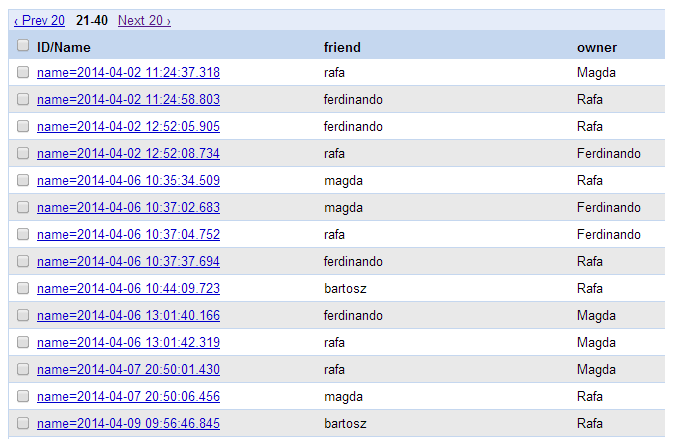
\includegraphics[scale=0.8]{figures/datastore.png}
	\end{center}
	
	\caption{Saved entries for the FriendFinder app}.
	\label{pic:dataviewer}

\end{figure}


\section{SensibleDTU data}

 The second type of data comes from the SensibleDTU data collector app. Based on \cite{Stopczynski}, we will give a short description of the project, with an emphasis on data collection. We will then focus on the actual data, its form, and how it was collected.	